\section{Tests}
\label{section:tests}

\subsection{Type of tests}

\subsubsection{JUnit}

\begin{figure}[h]
	\centering
	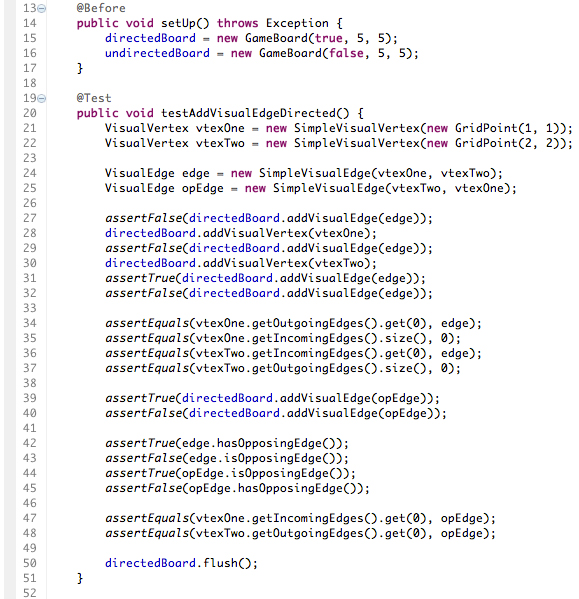
\includegraphics[width=.95\textwidth]{junit_screenshot.jpg}
	\caption{JUnit test for the GameBoard.}
	\label{img:screenJUnit}
\end{figure}
\emph{JUnit} is the most commonly used framework to write repeatable unit tests for Java applications.\par
Every object can be tested separately using defined input values and expected output values. Methods and object correlations not working as intended will attract attention reliably.\par
Fig. \ref{img:screenJUnit} shows a unit test implemented with JUnit. It verifies the correctness of the program when adding a new directed \emph{VisualEdge}.

\subsubsection{Algorithm regression tests}

\graphioli uses three graph algorithms: \emph{BreadthFirstSearch}, \emph{FindPath} and \emph{PlanarityCheck}\footnote{Only the planarity of a specific drawing is checked.}. Their unit tests are implemented with JUnit as well and are designed as regression tests to verify the algorithm's correct behavior.\par
In order to achieve the best possible code coverage and a high level of verification, the algorithms are fed with different combinations of input parameters, e.g. vertices at different grid positions, a variety of different graphs etc. Their output is verified agains the asserted results.\par

\textbf{BreadthFirstSearch}\par
Fig. \ref{img:bfsTestGraph} shows a graph that is used for testing the algorithm.\par
Starting at, for instance, vertex `1', BreadthFirstSearch is performed in different depths and the result is asserted against the expected values.\par
This is done in many different combinations and with \emph{positive} and \emph{negative} assertions: We verify that a specific result occurs and falsify that specific (invalid) results don't show up.\par

\begin{figure}[!h]
	\centering
	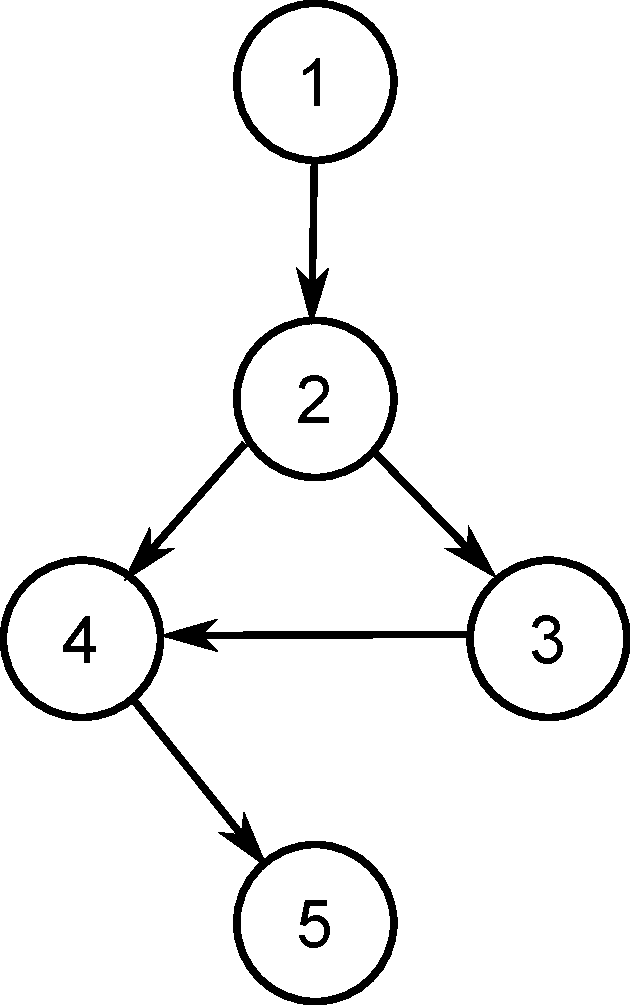
\includegraphics[scale=0.3]{bfsTestGraph.pdf}
	\caption{Graph used in several regression tests for the \emph{BreadthFirstSearch} algorithm.}
	\label{img:bfsTestGraph}
\end{figure}

\pagebreak
\textbf{FindPath}\par
This algorithm heavily bases on \emph{BreadthFirstSearch} and is tested in the same way.\par

\textbf{PlanarityCheck}\par
Fig. \ref{img:planarityTestGraph} visualizes a graph that is used for the automated \emph{PlanarityCheck} tests. Those tests feed the algorithm with different planar and non-planar drawings. The algorithm's output is then verified against the graph's actual properties.\par

\begin{figure}[!h]
	\centering
	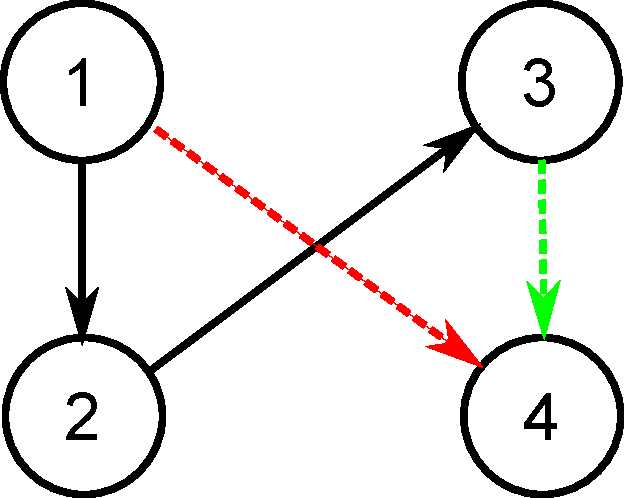
\includegraphics[scale=0.3]{planarityTestGraph.pdf}
	\caption{Visualization of the \emph{testPerformAlgorithm} method that is used for testing the \emph{PlanarityCheck} algorithm.}
	\label{img:planarityTestGraph}
\end{figure}


\subsubsection{Sikuli}

\begin{figure}[!h]
	\centering
	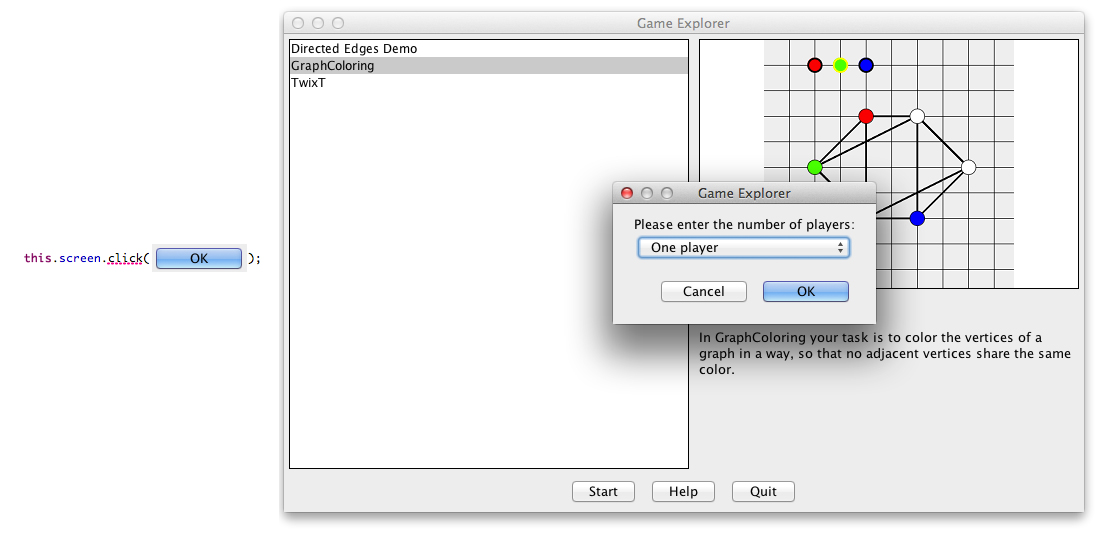
\includegraphics[width=.95\textwidth]{sikuli_click.jpg}
	\caption{Sikuli looks for the specified screenshot crop (in this case the `OK' button) in the GUI element.}
	\label{img:screenSikuli1}
\end{figure}
\begin{figure}[!h]
	\centering
	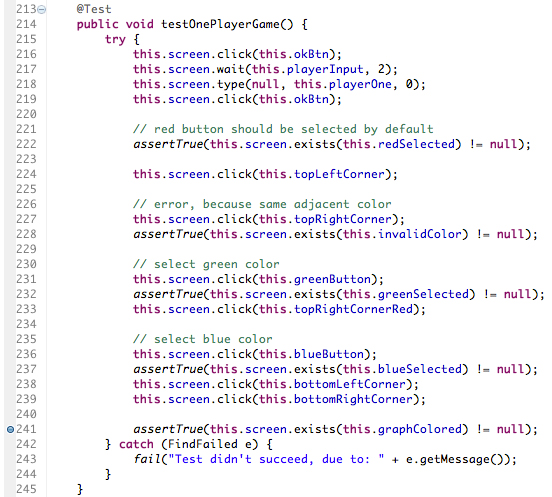
\includegraphics[width=.95\textwidth]{sikuli_screenshot_2.jpg}
	\caption{Sikuli test for the Graph-Coloring single-player game.}
	\label{img:screenSikuli2}
\end{figure}
\begin{figure}[!h]
	\centering
	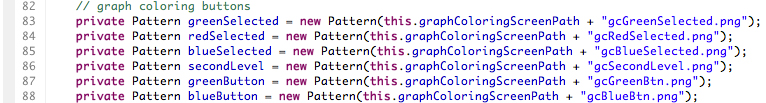
\includegraphics[width=.95\textwidth]{sikuli_screenshot_1.jpg}
	\caption{GUI elements defined for tests with Sikuli.}
	\label{img:screenSikuli3}
\end{figure}
For extensive tests of our graphical user interfaces (GUIs), we drew on open-source \emph{Project SIKULI}. Sikuli is a visual technology to automate and test those interfaces using screenshots.\par
Sikuli itself is written in Java and is being used by importing the Sikuli library.\par
With Sikuli every possible item can be clicked on, no matter if its a real button, text field or list item. The program simply looks for the provided screenshot in the GUI (see Fig. \ref{img:screenSikuli1}) and simulates a mouse click or key stroke on the item that it found. In Java code the test developer then defines click paths, key input and assertions. An example for this is outlined in Fig. \ref{img:screenSikuli2}.\par
Those assertions again are cropped images from screenshots. If they appear somewhere after the click, the test passes, otherwise it fails.\par
Once all clickable items are saved as screenshot parts (see Fig. \ref{img:screenSikuli3}), every possible scenario can be executed semi-automatically. These tests can also be designed as regression test.\par
With Sikuli one can only test visual existence or non-existence of a given object. For example if the execution of the help page calls 10 different methods, Sikuli is not able to test if the methods are correct, but can only verify if the end result is as expected.\par

\subsubsection{Manual tests}

As defined in the \emph{Functional Specifications Document}, we conducted 18 test cases and four test scenarios. As those have been defined before design and implementation, they give some indication of whether the framework and the games in general have been deployed as planned.\par

\subsection{Implementation details}
We implemented a lot of unit tests during our implementation phase, however possible errors could be embedded in the GUIs as well. And as Java does not provide easy and free frameworks for GUI testing, we used the above described Sikuli to act out almost all possible click and key combinations in both \gameexplorer and \emph{GameWindow}.\par
The - mainly positive - results of all tests are outlined in the next sections.\par
